\documentclass[10pt]{article}
\usepackage{graphicx}
\usepackage{amssymb}
\usepackage[fleqn]{amsmath}
\usepackage{nccmath}
\usepackage{cases}
\usepackage{hyperref}
\usepackage{multicol}
\usepackage{tikz}
\usepackage{tikz}
\usetikzlibrary{shapes.geometric}
\usepackage{pgfplots}
\usepackage{enumitem}
\pgfplotsset{compat=1.18}
\usepackage{float}

\title{\bf Math 106: Problem Set 2}
\date{1/28/2024}
\author{\bf Owen Jones}
\begin{document}
\maketitle
\begin{enumerate}
    \item [\textbf{2.1.1}] \begin{enumerate}
        \item [CN4.] In symbolic notation, we have $a=b\Rightarrow a\cong b$. 
        We make the assumption that anything coincides with itself. 
        Thus, by CN4, $a=a\Rightarrow a\cong a$, so we obtain the reflexive property. 
        Hence, CN4 can be interpretted as the reflexive property.
        \item [CN1.] In symbolic notation, we have $a\cong c\land b\cong c\Rightarrow a\cong b$. 
        In 2.1.2, we show that the symmetric property follows from CN1 and CN4. 
        Suppose $a\cong b\land c\cong b$. 
        It follows by the symmetric property we also have $a\cong b\land b\cong c$. 
        By CN1, we have $a\cong b\land b\cong c\Rightarrow a\cong c$.
        Hence, CN1 can be interpretted as the transitive property.
    \end{enumerate}
    \item [\textbf{2.1.2}] Suppose $a\cong b$. 
    By CN1 we have $b\cong b$. 
    By CN4, we have $b\cong b\land a\cong b\Rightarrow b\cong a$.
    Hence, $a\cong b\Rightarrow b\cong a$.
    \item [\textbf{2.2.1}] WLOG let each side of the cube and octahedron be $1$ unit in length. 
    The distance from the center of the cube to the center of any face is half the length of the side length, $\frac{1}{2}$.
    It follows the inradius is $\frac{1}{2}$. 
    By the Pythagorean Theorem, the distance from the center to any vertex is $\sqrt{\frac{1^2}{2^2}+\frac{1^2}{2^2}+\frac{1^2}{2^2}}=\frac{\sqrt{3}}{2}$.
    It follows the circumradius is $\frac{\sqrt{3}}{2}$.
    Hence, $\frac{circumradius}{inradius}=\sqrt{3}$.\\
    By similar triangles, the distance from the center of the octahedron to the center of any face is $\frac{r}{\frac{1}{2}}=\frac{\frac{\sqrt{2}}{2}}{\frac{\sqrt{3}}{2}}\Rightarrow r=\frac{\sqrt{6}}{6}$.
    By the Pythagorean Theorem, the distance from the center of the octahedron to any vertex is $\sqrt{1-\frac{\sqrt{3}}{2}}=\frac{\sqrt{2}}{2}$.
    Hence, $\frac{circumradius}{inradius}=\frac{\frac{\sqrt{2}}{2}}{\frac{\sqrt{6}}{6}}=\sqrt{3}$.
    \item [\textbf{2.2.2}] $CA=\sqrt{{(\frac{\phi-1}{2})}^2+{(\frac{1}{2})}^2+{(\frac{\phi}{2})}^2}=\frac{\sqrt{2\phi^2-2\phi+2}}{2}=\frac{\sqrt{2(\phi+1)-2\phi+2}}{2}=\frac{\sqrt{4}}{2}=1$.\\
    \begin{figure}[H]
        \includegraphics{Screenshot 2024-01-28 at 2.06.50 PM.png}
    \end{figure}
    We solve for $AB$ in the same way we solve for $CA$. Thus, $AB=BC=CA=1$.
    \item [\textbf{2.3}] Problems in section 2.3 are done on pencil and paper.
    \item [\textbf{2.4.1}] The string is some length $l$. 
    Place the pins at points $F_1$ and $F_2$ that are distance less than $l$ away from each other. 
    Attach the ends of the string to the pins. 
    Place a pen or pencil on the inside of the string and move away from the semi-major axis until the string is taut.
    Trace a path around the pins that keeps tension on the string at all times. 
    The resulting shape should be an ellipse.
    \item [\textbf{2.4.2}] Let the two foci be located at $(c,0)$ and $(-c,0)$ with the extremal points being $(a,0),(-a,0),(b,0),(-b,0)$. 
    Because the sum of the distances from each foci to a point is constant, we obtain $2|a|=2\sqrt{b^2+c^2}\Rightarrow c^2=a^2-b^2$.
    Thus, for any point on the ellipse, $\sqrt{{(x-c)}^2+y^2}+\sqrt{{(x+c)}^2+y^2}=2a$.\\
    ${(x-c)}^2+y^2=4a^2-4a\sqrt{{(x+c)}^2+y^2}+{(x+c)}^2+y^2\\
    \Rightarrow 4cx+4a^2=4a\sqrt{{(x+c)}^2+y^2}\\
    \Rightarrow c^2x^2+2a^2cx+a^4=a^2x^2+2a^2cx+a^2c^2+a^2y^2\\
    \Rightarrow (a^2-b^2)x^2+a^4=a^2x^2+a^2(a^2-b^2)+a^2y^2\\
    \Rightarrow a^2b^2=b^2x^2+a^2y^2\\
    \Rightarrow\frac{x^2}{a^2}+\frac{y^2}{b^2}=1$
    \begin{figure}
        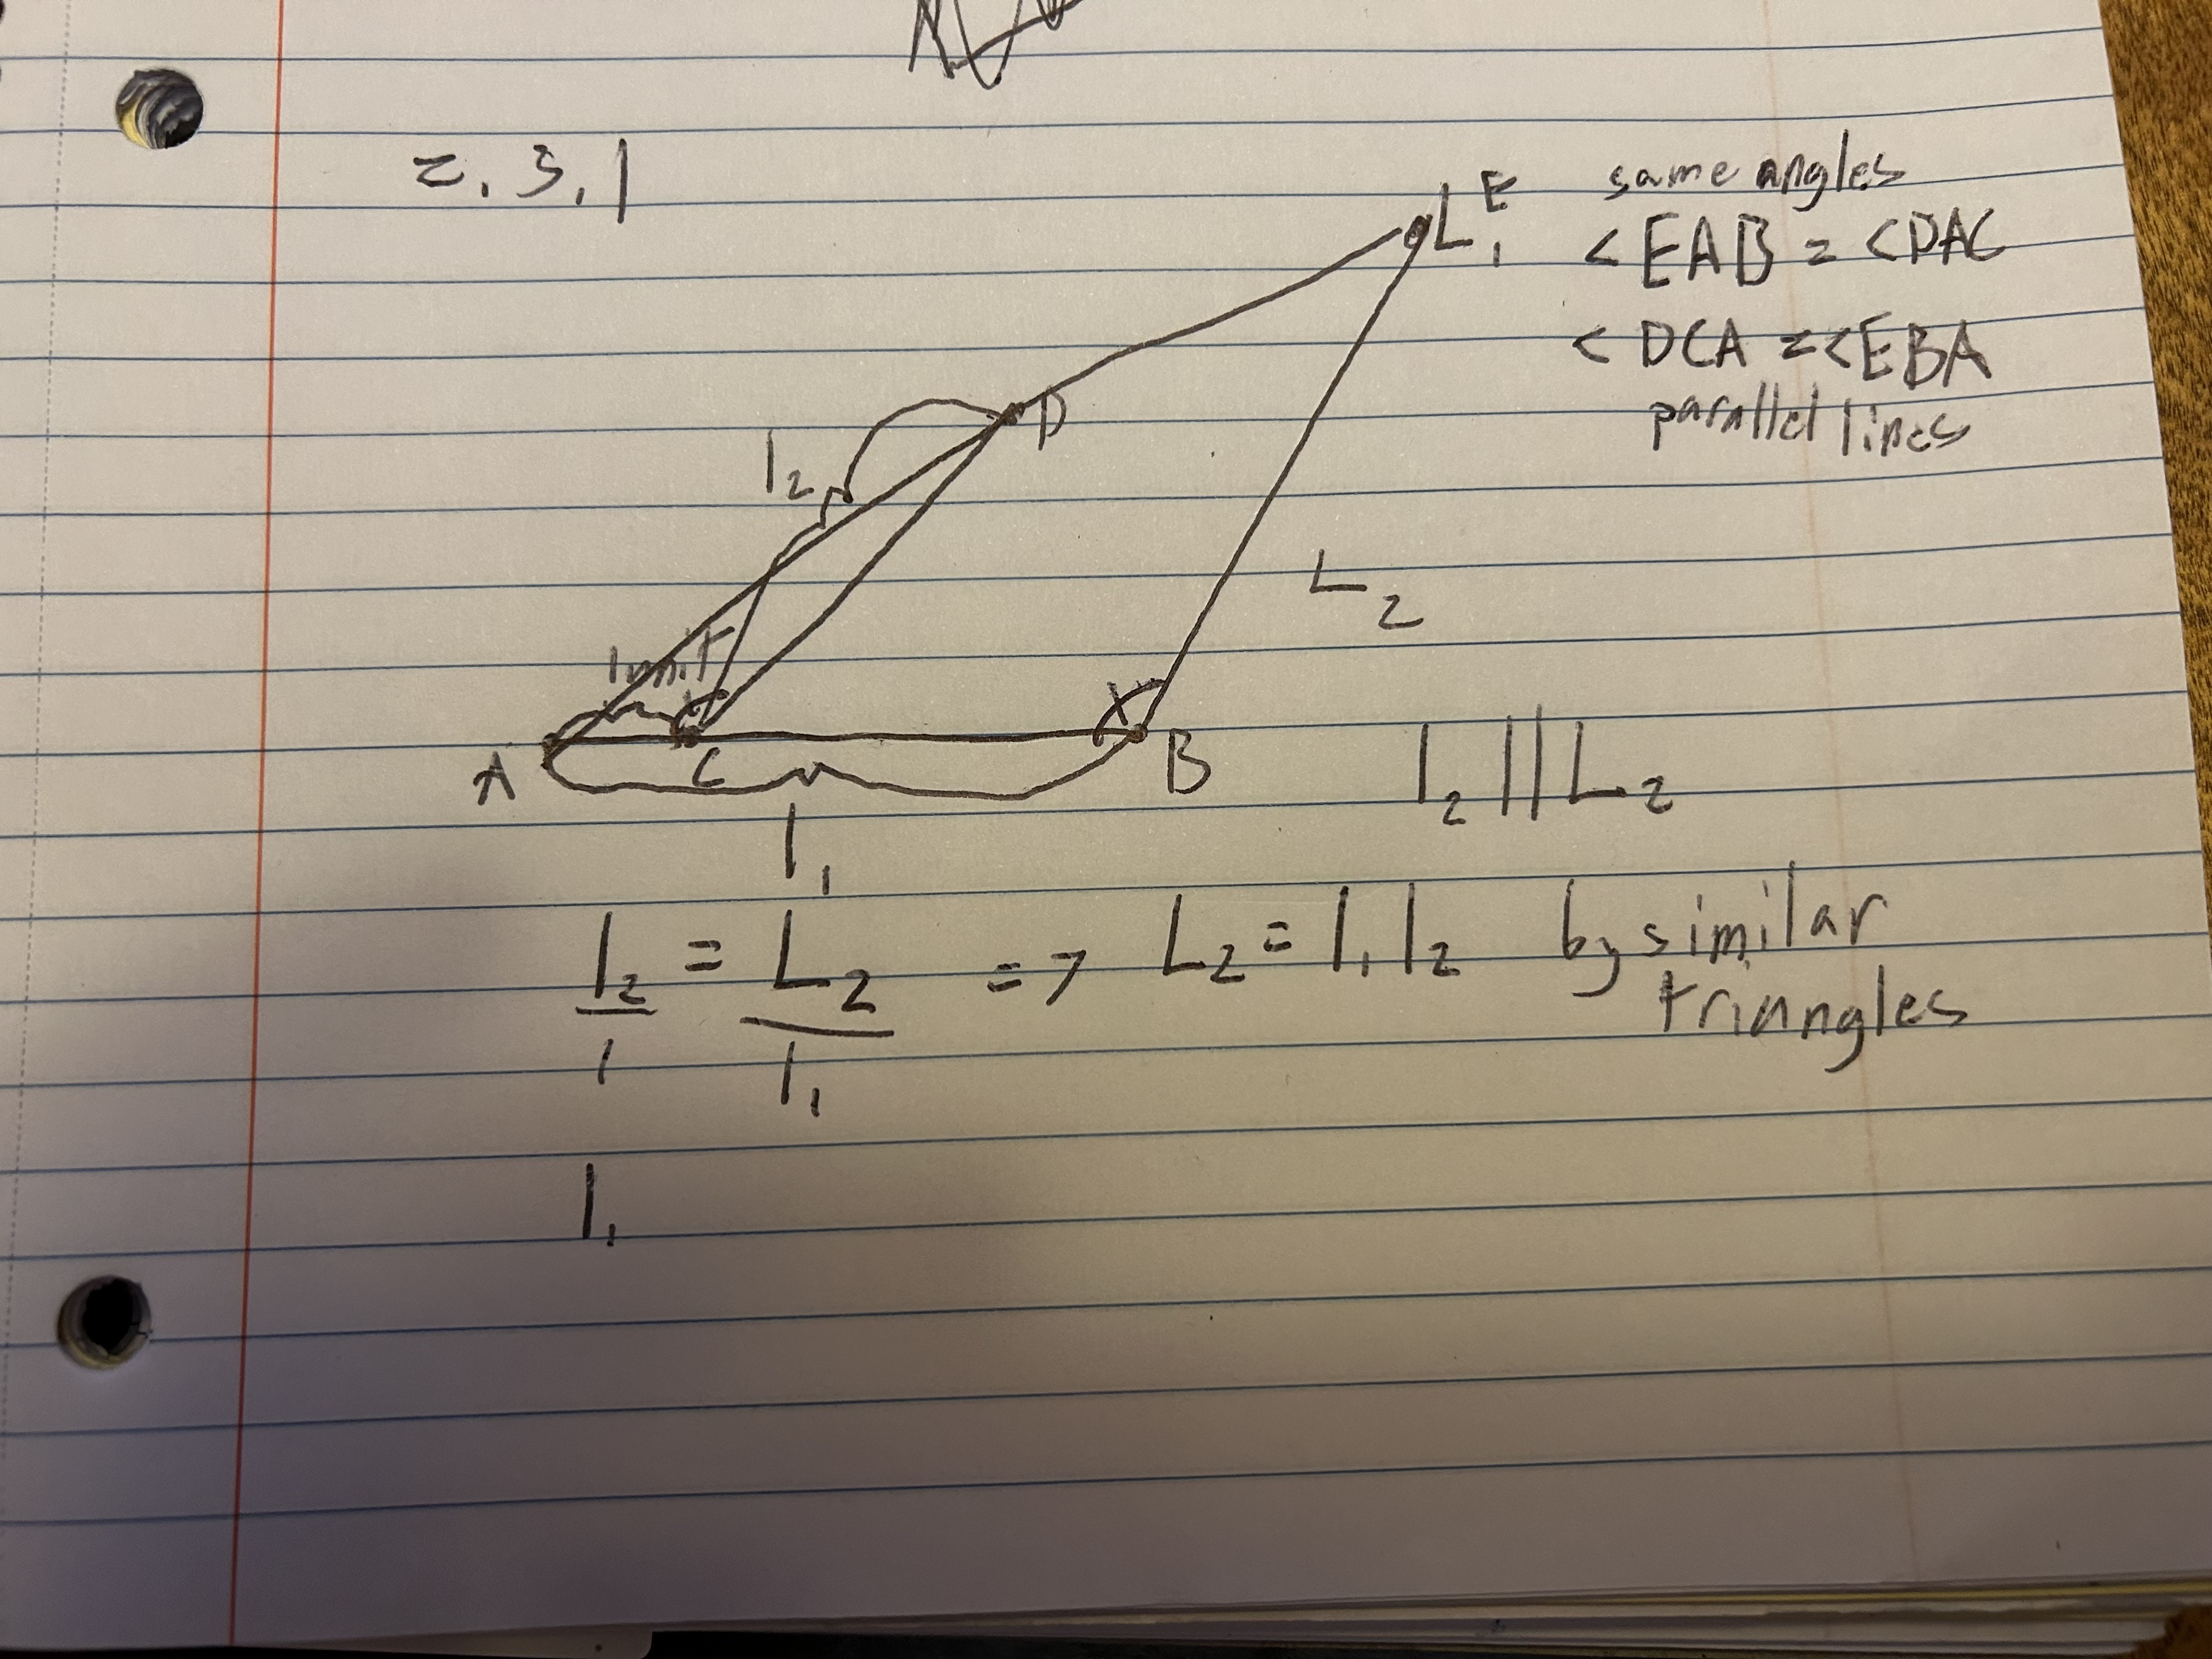
\includegraphics[scale=0.1]{IMG_0674}
    \end{figure}
    \begin{figure}
        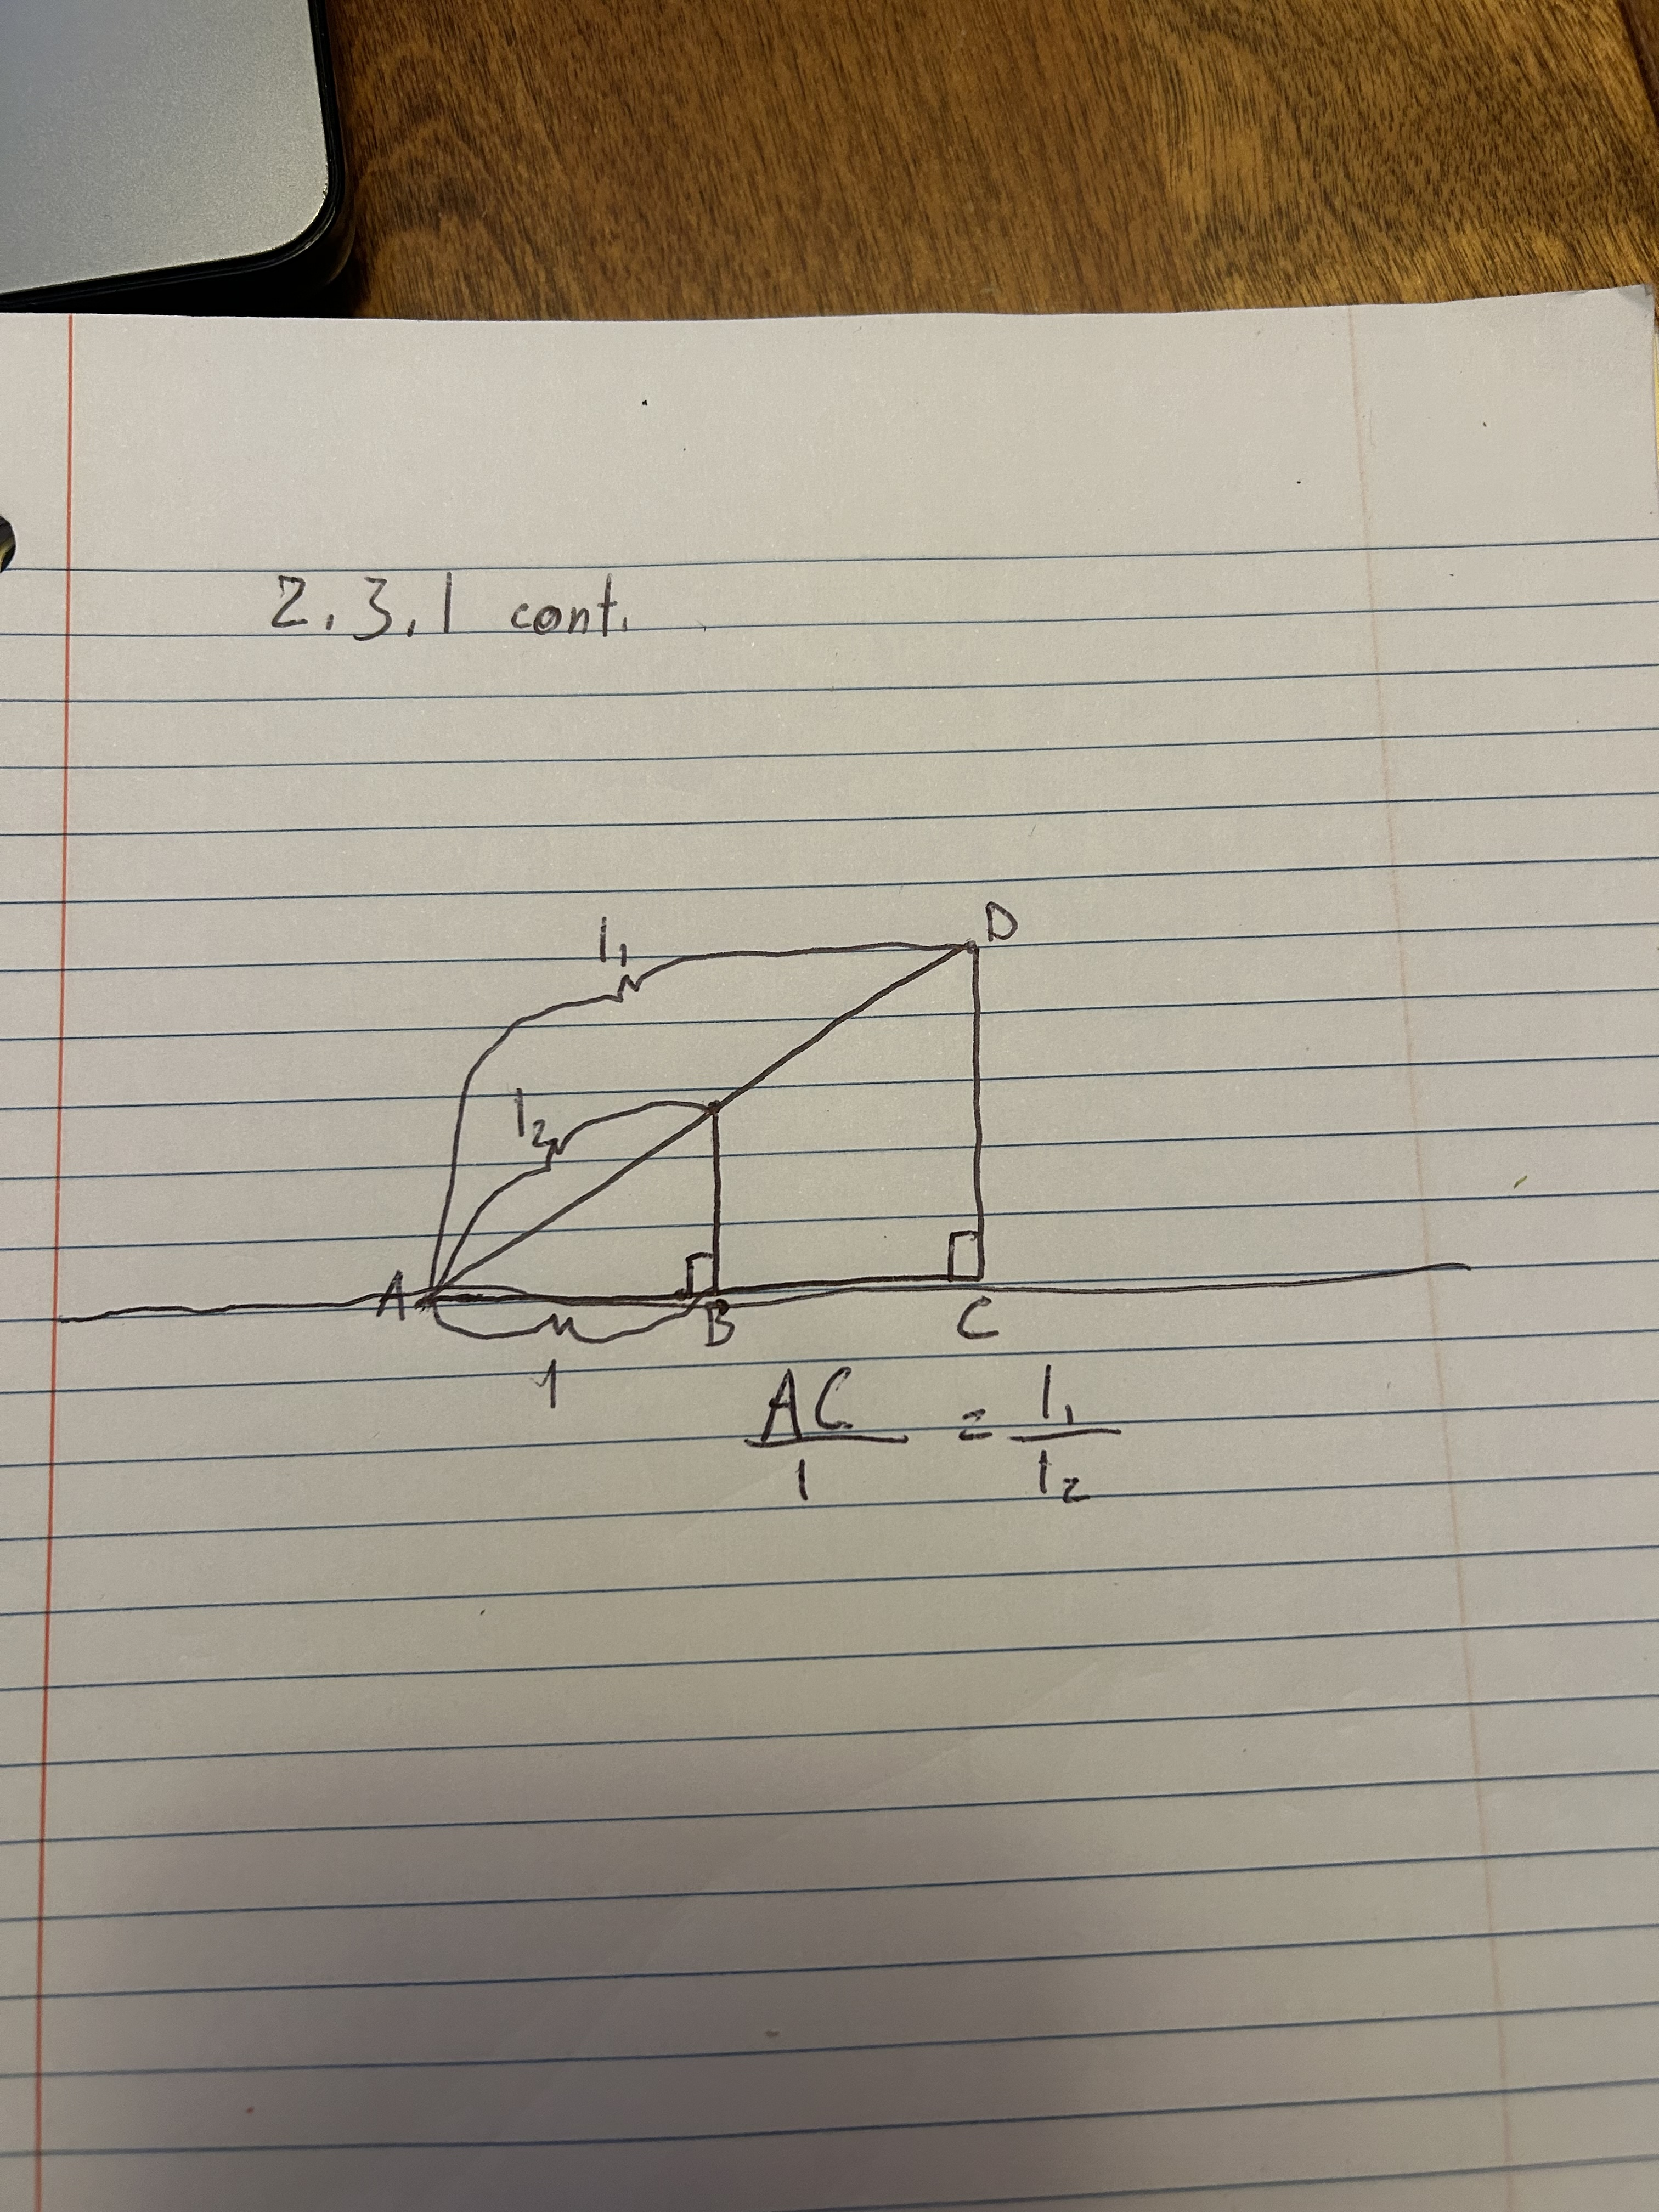
\includegraphics[scale=0.15]{IMG_0675}
    \end{figure}
    \begin{figure}
        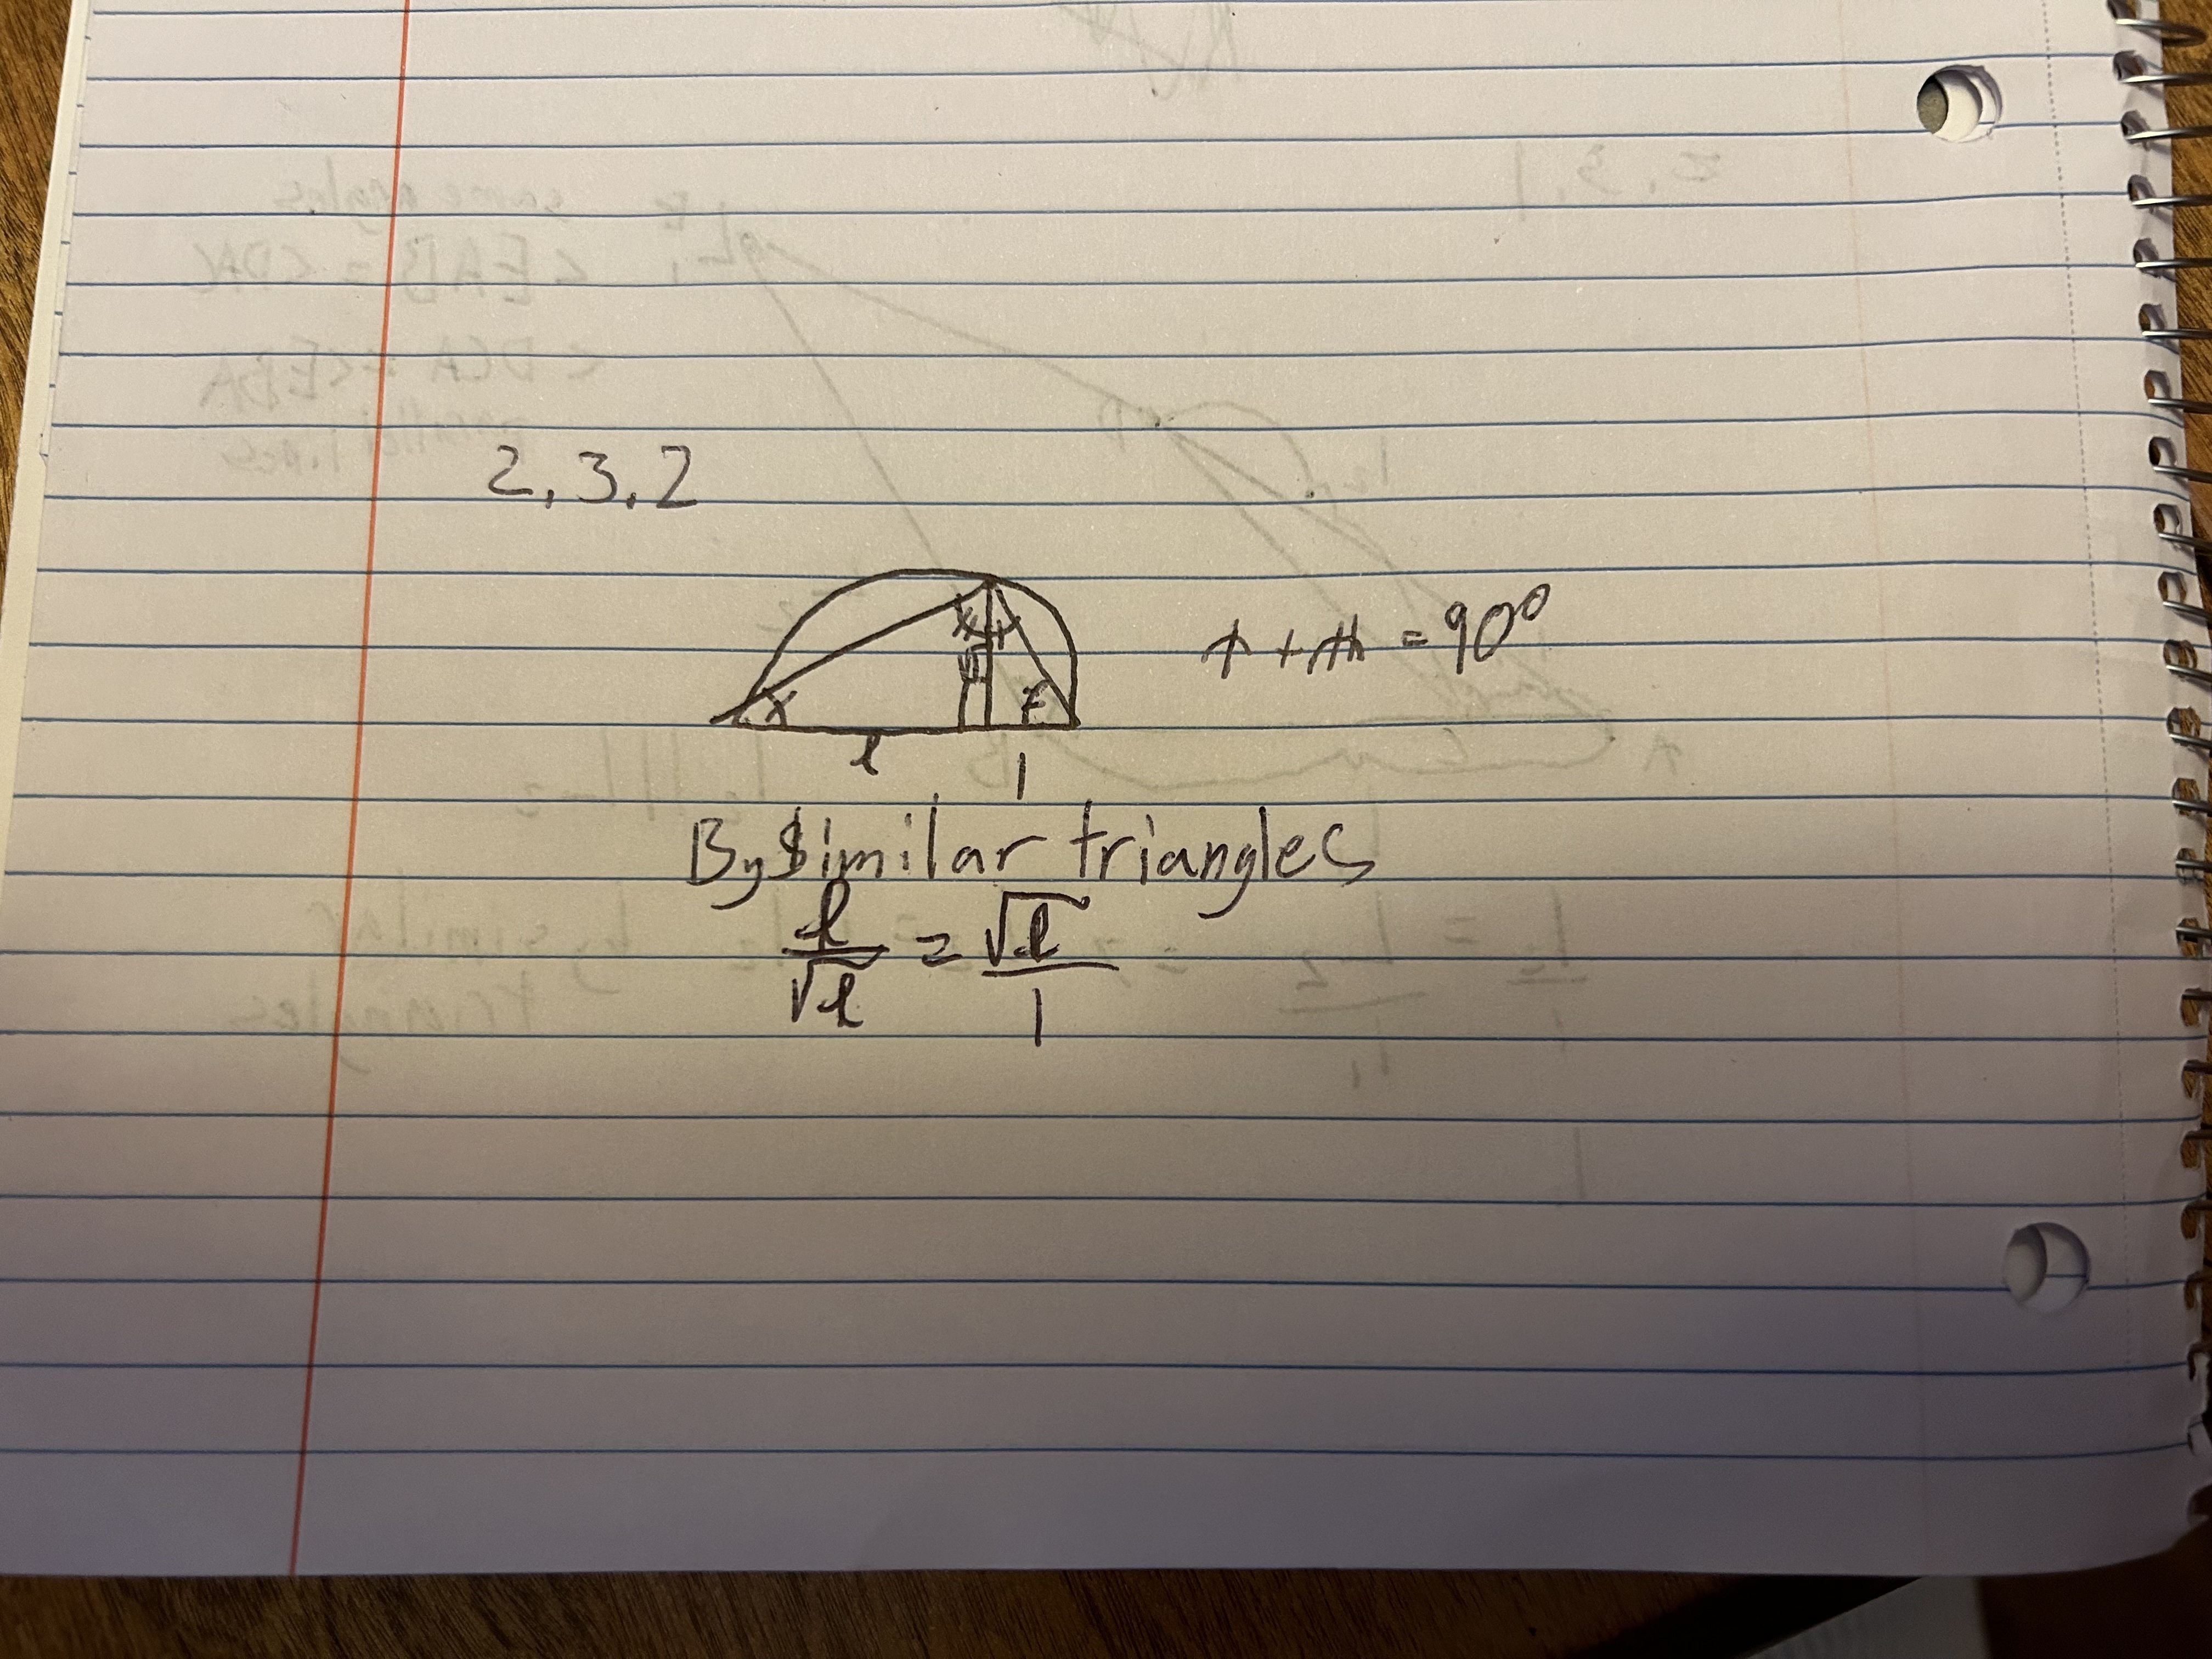
\includegraphics[scale=0.1]{IMG_0676}
    \end{figure}
    \begin{figure}
        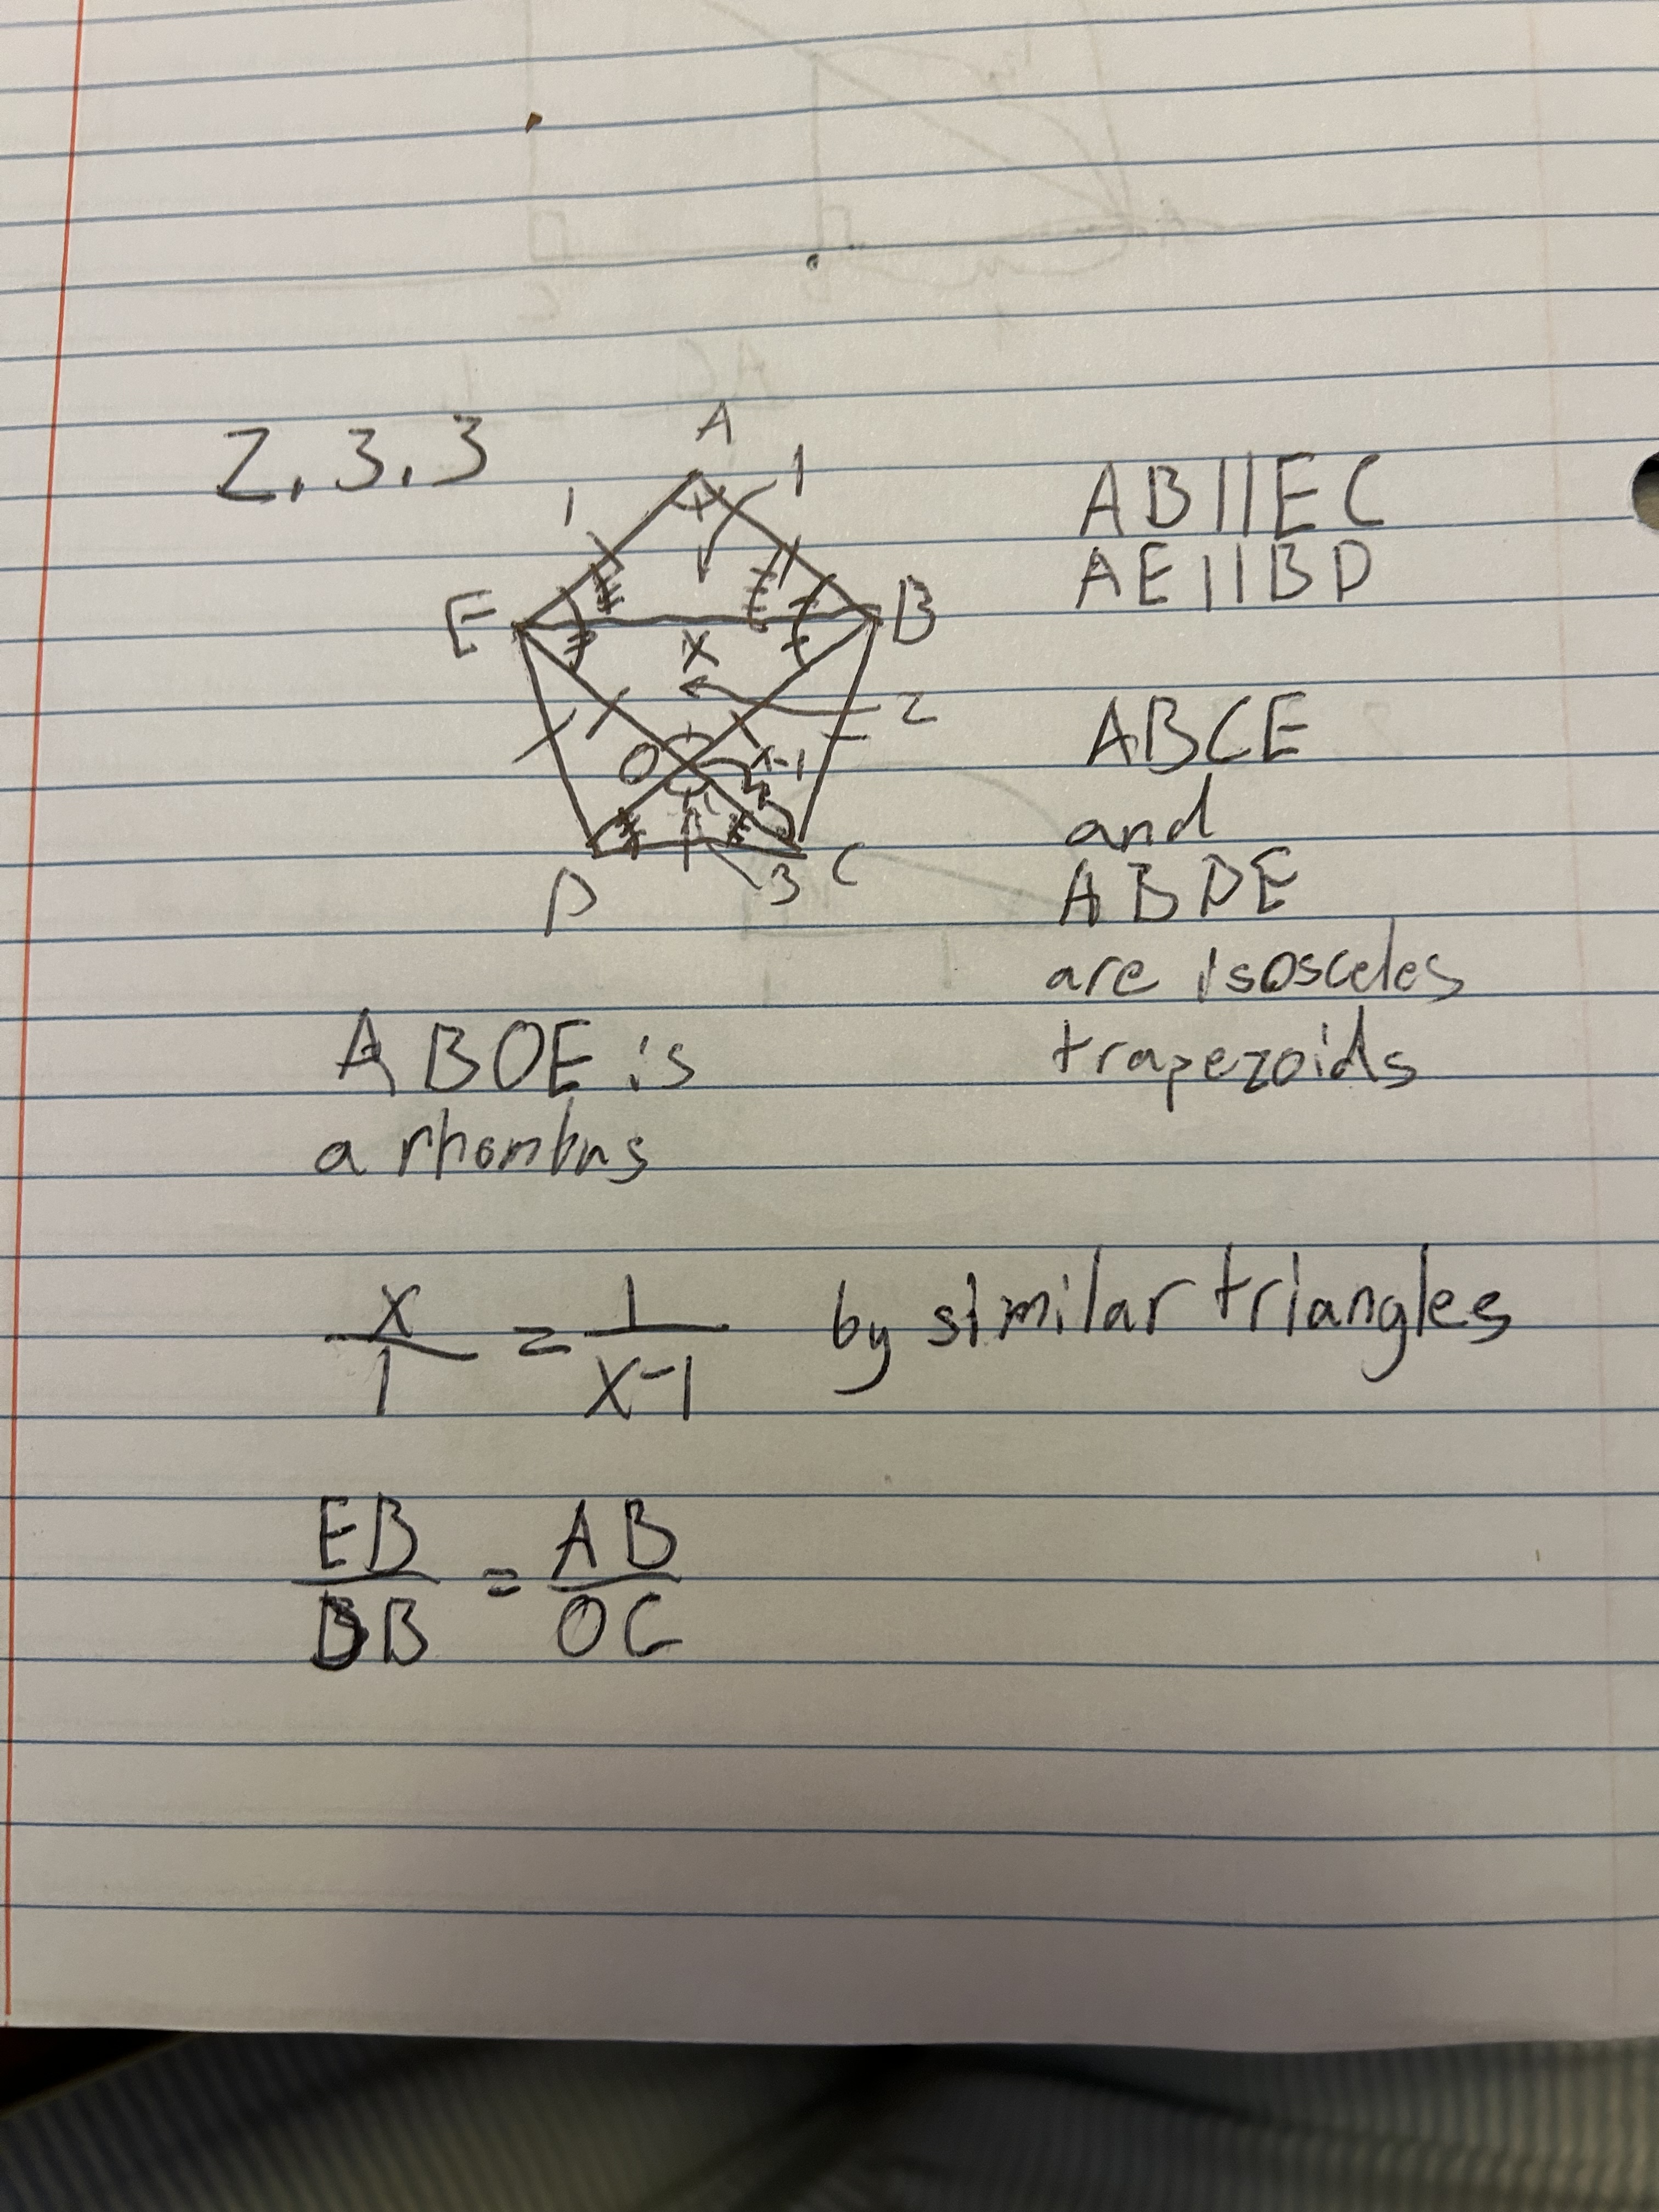
\includegraphics[scale=0.15]{IMG_0679}
    \end{figure}
    \begin{figure}
        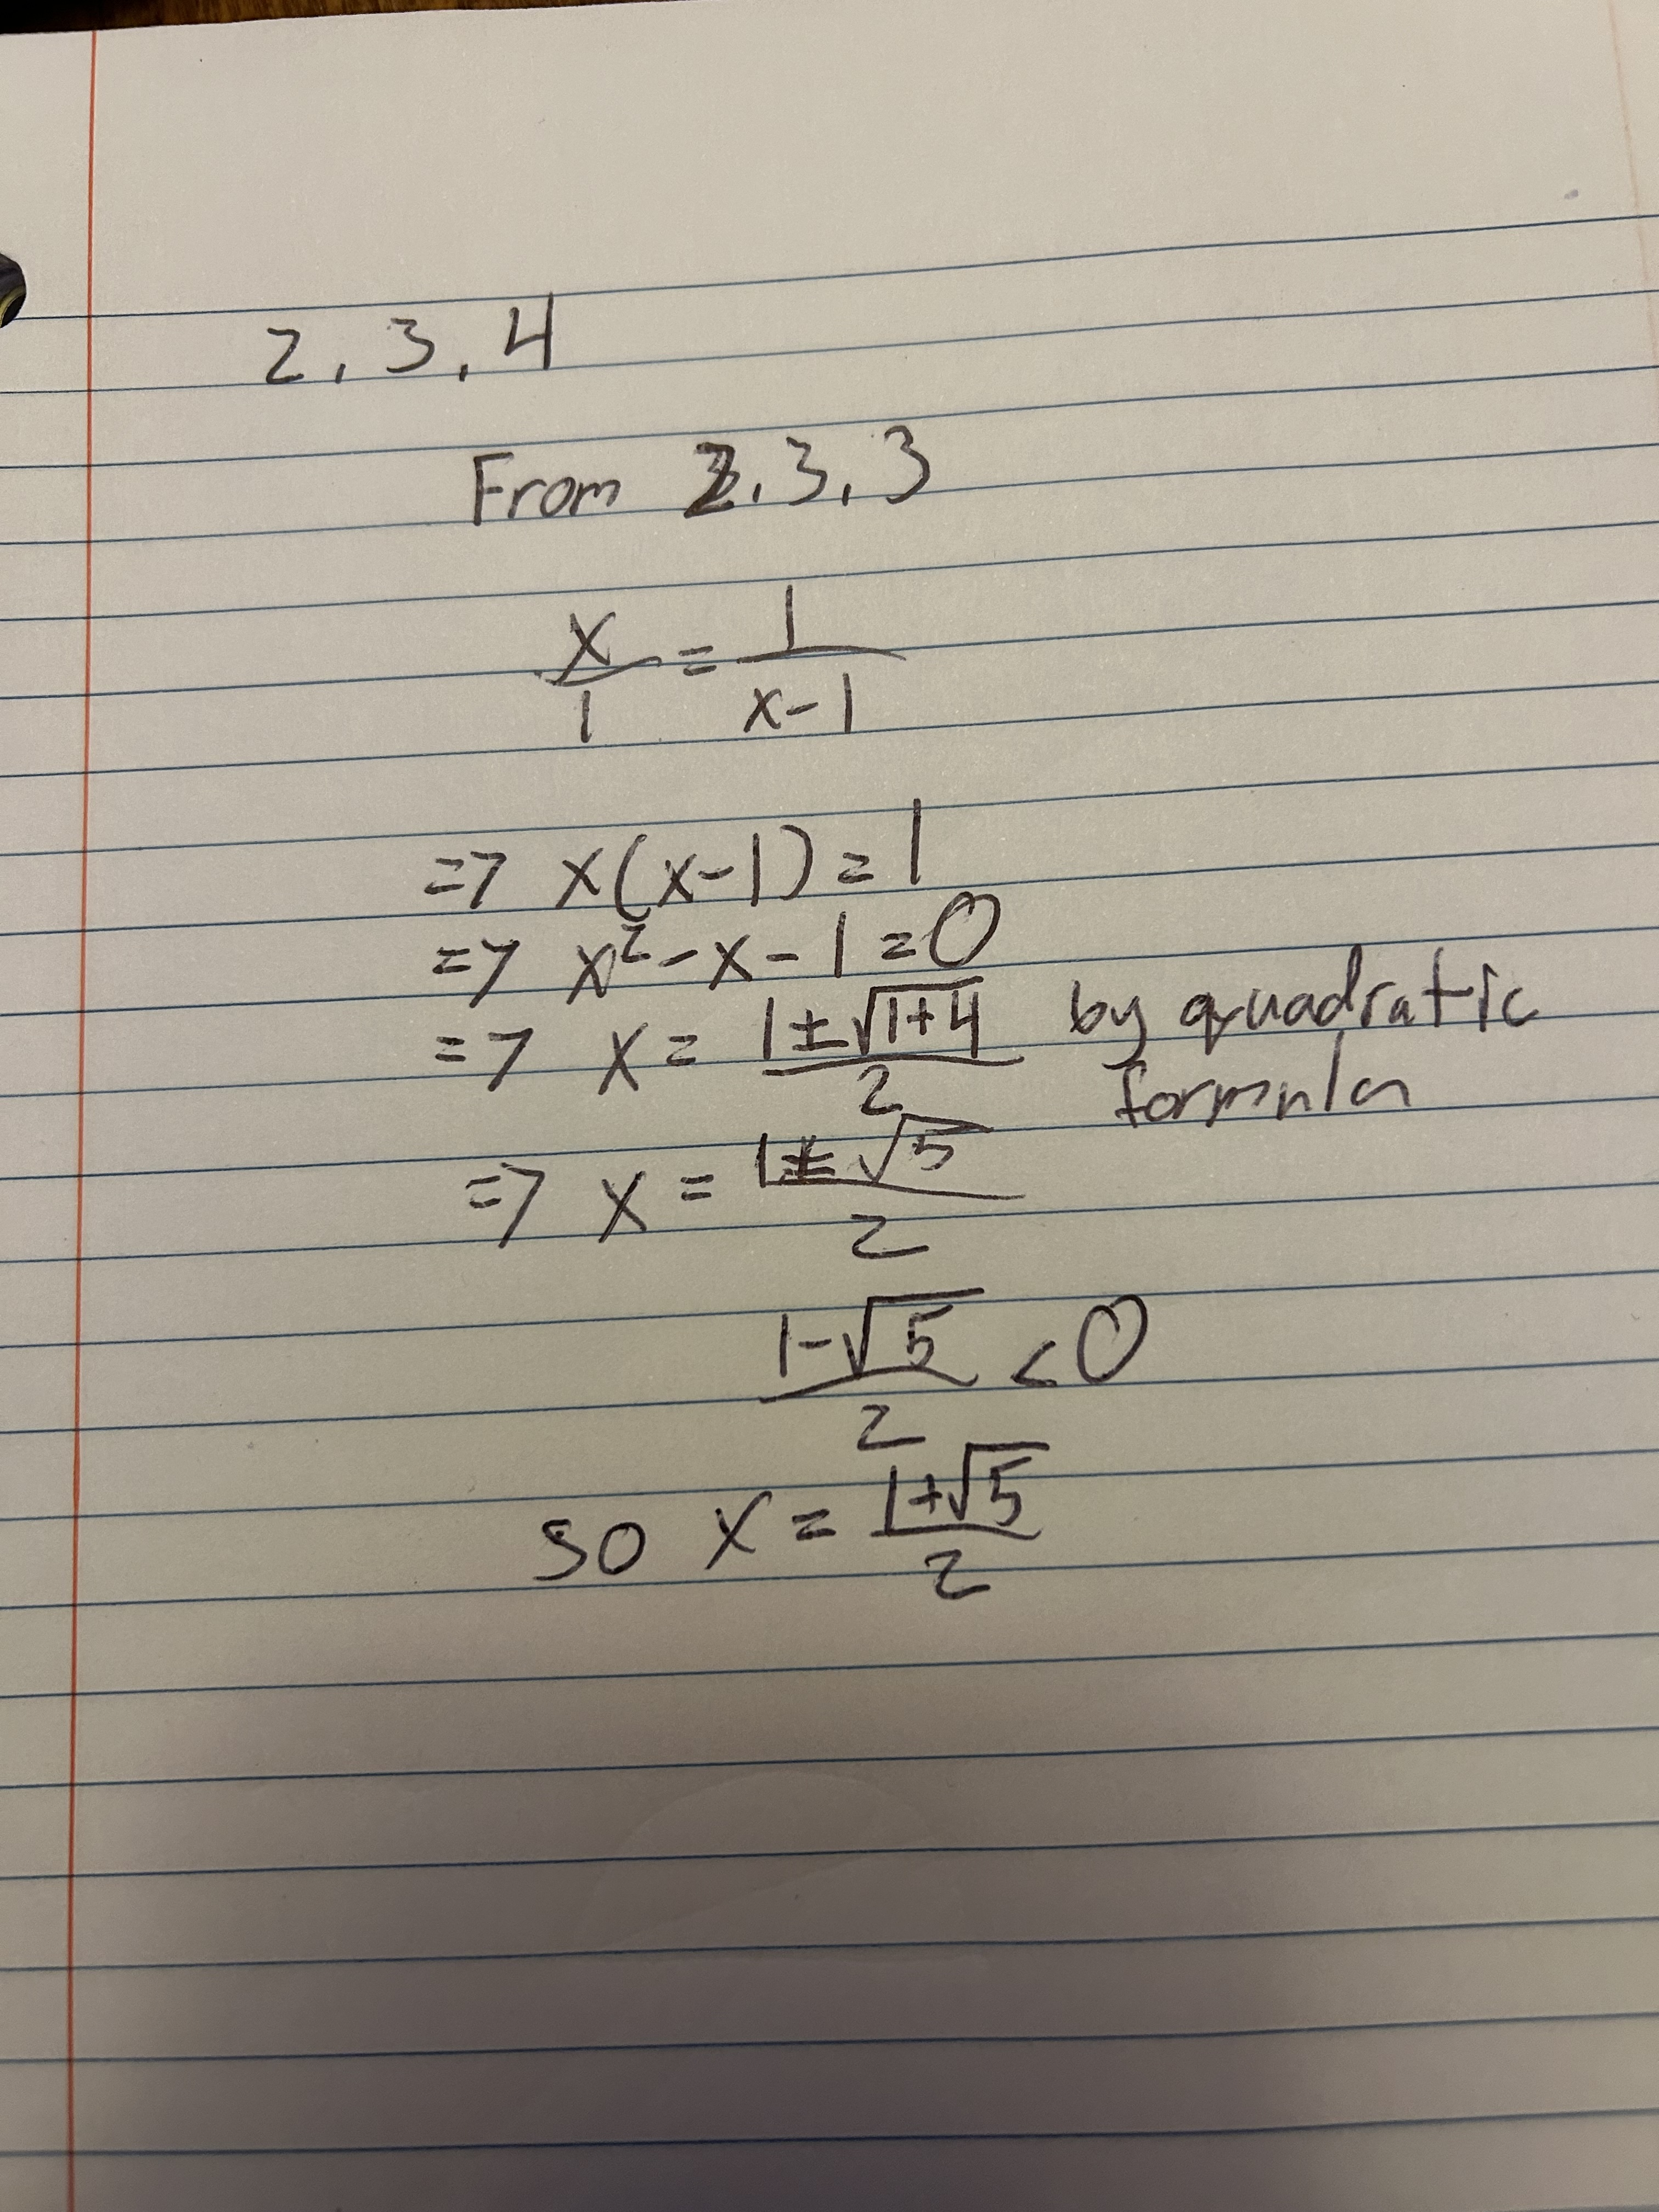
\includegraphics[scale=0.15]{IMG_0678}
    \end{figure}
\end{enumerate}
\end{document}